% Opener for November 11, 2026: whose pile? (who has which pile of counters)
% Build in a scratch directory: pdflatex whose-pile.tex, then copy the PDF to ../2026-11-11-opener.pdf
% Every puzzle here is checked for exactly one answer by whose-pile_check.py.
\documentclass[11pt]{article}
\usepackage[letterpaper,margin=0.5in]{geometry}
\usepackage[T1]{fontenc}
\usepackage[default]{sourcesanspro}
\usepackage{tikz}
\pagestyle{empty}
\setlength{\parindent}{0pt}
% \pile{y}{n}: a row of n counters at height y, then a line to write the animal's name
\newcommand{\pile}[2]{%
  \foreach \i in {1,...,#2} \draw[fill=gray!25,line width=0.8pt] (\i*0.62-0.31,#1) circle (0.24);
  \node[anchor=west,font=\large] at (5.3,#1) {#2 counters};
  \draw[line width=0.6pt] (7.8,#1-0.2) -- ++(5.4,0);}
\newenvironment{half}{\begin{minipage}[t][0.475\textheight][t]{\linewidth}\large}{\end{minipage}}
\newcommand{\cutline}{\par\noindent\begin{tikzpicture}\draw[dashed,gray] (0,0)--(\linewidth-0.4pt,0);\end{tikzpicture}\par\vspace{0.3in}}
\newcommand{\heading}[1]{{\LARGE\bfseries #1}\par\medskip}
\newcommand{\mainpuzzle}{%
  \heading{Whose pile?}
  Duck, Frog, Goat and Mouse each have a pile of counters.
  Write each animal's name next to its pile.
  \begin{center}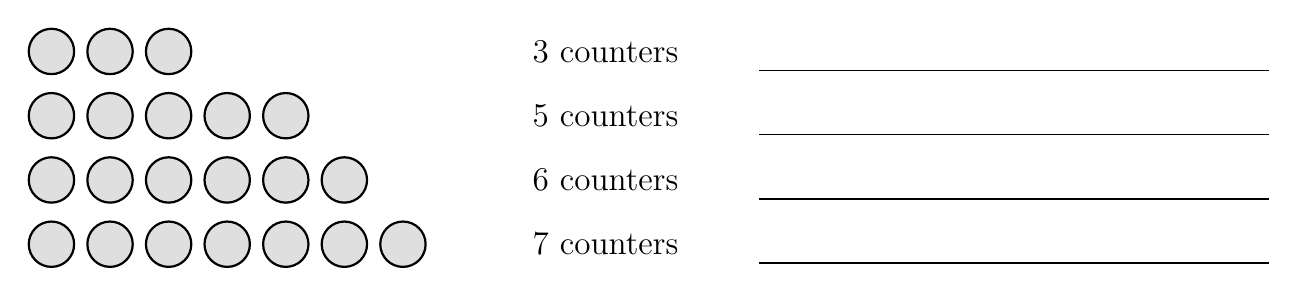
\begin{tikzpicture}[scale=1.2]
    \pile{0}{3}\pile{-0.68}{5}\pile{-1.36}{6}\pile{-2.04}{7}\end{tikzpicture}\end{center}
  \begin{enumerate}\setlength{\itemsep}{2pt}
  \item Frog has an odd number of counters.
  \item Mouse has fewer counters than Frog.
  \item Goat has more counters than Frog.
  \item Duck does not have the biggest pile.
  \end{enumerate}
  \textbf{Done?} Cross out clue 4. How many answers are there now? Write a new clue that makes it exactly one again.}
\begin{document}
\begin{half}\mainpuzzle\end{half}
\cutline
\begin{half}\mainpuzzle\end{half}
\newpage
\begin{half}
\heading{Whose pile? (three animals)}
Frog, Goat and Mouse each have a pile of counters.
Write each animal's name, or its first letter, next to its pile.
\begin{center}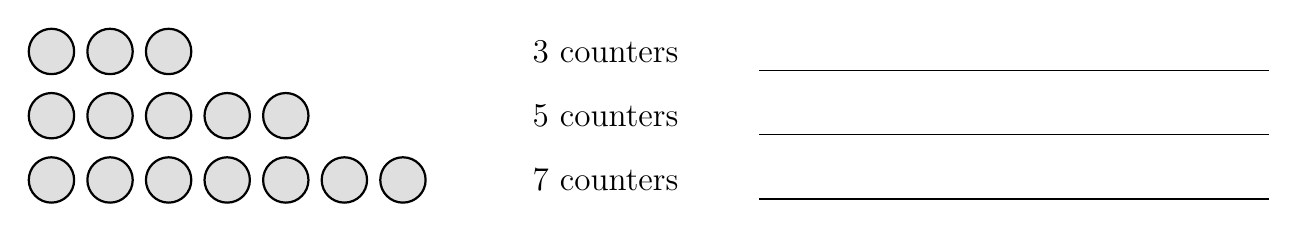
\begin{tikzpicture}[scale=1.2]
  \pile{0}{3}\pile{-0.68}{5}\pile{-1.36}{7}\end{tikzpicture}\end{center}
\begin{enumerate}\setlength{\itemsep}{2pt}
\item Goat has the most counters.
\item Mouse has fewer counters than Frog.
\end{enumerate}
\textbf{Done?} Try the four-animal puzzle.
\end{half}
\cutline
\begin{half}
\heading{Whose pile? (five animals)}
Duck, Frog, Goat, Hen and Mouse each have a pile of counters.
Write each animal's name next to its pile.
\begin{center}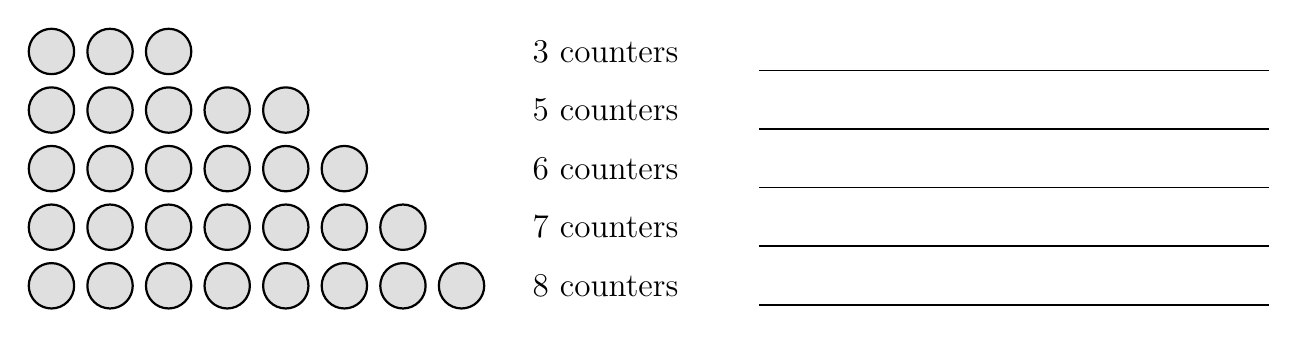
\begin{tikzpicture}[scale=1.2]
  \pile{0}{3}\pile{-0.62}{5}\pile{-1.24}{6}\pile{-1.86}{7}\pile{-2.48}{8}\end{tikzpicture}\end{center}
\begin{enumerate}\setlength{\itemsep}{1pt}
\item Duck has an even number of counters.
\item Hen has an even number of counters.
\item Hen has more counters than Duck.
\item Frog has exactly two more counters than Mouse.
\item Goat has more counters than Frog.
\end{enumerate}
\textbf{Done?} Write your own pile puzzle with exactly one answer, and give it to a friend.
\end{half}
\end{document}
